\documentclass[conference]{IEEEtran}
\usepackage[utf8]{inputenc}
\usepackage{amssymb}
\usepackage{graphicx}
\usepackage{pifont}
\usepackage{multirow}
\newcommand{\cmark}{\ding{51}}%

\title{Aduno: Real-Time Collaboration and Articulation in Shared Workspaces}
\author{\IEEEauthorblockN{Braden Simpson}
\IEEEauthorblockA{University of Victoria\\
Victoria, British Columbia\\
braden@uvic.ca}
\and
\IEEEauthorblockN{Eirini Kalliamvakou}
\IEEEauthorblockA{University of Victoria\\
Victoria, British Columbia\\
ikaliam@uvic.ca}
\and
\IEEEauthorblockN{Nathan Lambert}
\IEEEauthorblockA{University of Victoria\\
Victoria, British Columbia\\
nlambert@uvic.ca}}

\begin{document}
\maketitle

\begin{abstract}
Awareness is considered one of the most critical elements of collaborative activities, and to achieve and maintain it collaborators need to establish common ground while working together. In distributed software development, the concept of awareness has been researched extensively and there is a plethora of tools to support it. We introduce Aduno, a tool that enables real-time articulation work for software development tasks, and helps with creating and maintaining common ground between software developers as they define work items. In line with the growing adoption of GitHub, Aduno also links to GitHub's issue tracker to easily translate work items on a whiteboard to project work items.
\end{abstract}

\section{Introduction \& Motivation}
\label{sec:intro}

Teams today, especially as they become distributed, need {\sc cscw} applications that support them through all phases of their collaboration by providing them with the essential context. Successful collaboration between members of a distributed team requires that people are aware of each others' actions and that they maintain this awareness so that there are as few disruptions as possible in their workflow and their coordination. One setting that these principles take effect in is distributed software development, where teams need to coordnate for different sets of activities until they have built the end product. We introduce a shared workspace application for task creation and articulation work in software development teams. Our solution successfully supports workspace awareness and grounding as a collaborative basis in a development project, while exporting work items as issues on GitHub.

To be able to effectively support workspace awareness through tools, we first need insight on how people maintain awareness. One of the most influential approaches is Neisser's Perception-Action Cycle \cite{Neisser76} which was developed to describe the interaction between a person, the environment and its effects on perception, especially as new information is added to the environment.  This can be seen in Figure~\ref{fig:neisser}. A person entering an environment to perform a task, brings an understanding of the situation and what they are looking for. They acquire information from the environment which they interpret in light of their existing knowledge, and use it to reevaluate the state of the environment. This new knowledge also directs a person's predictions about a future state of their environment and shapes the  ir perception of it. Awareness of the environment a person operates in translates into gathering information and using that to constantly make decisions about their next move. For collaborating teams, having access to the information that allows members to make these decisions is crucial.

%TODO a bit more on this

\begin{figure}[htb]
\centering
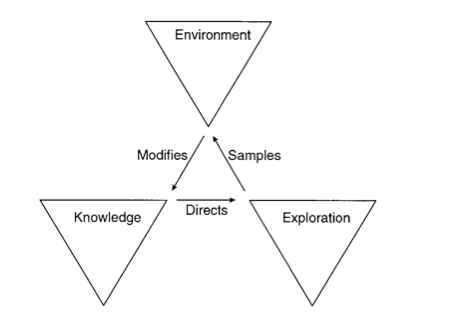
\includegraphics[scale=0.5]{neisser}
\caption{Neisser's Perception-Action Cycle}
\label{fig:neisser}
\end{figure}

In physical workspaces it is easy for collaborators to maintain awareness by interpreting visual and audio stimuli. People working in the same office or in open spaces can easily get information on others' work progress or tasks they are involved in. Virtual workspaces, however, face restrictions in terms of this kind of inferred knowledge, and with limited information, awareness is hindered. Gutwin et al.~\cite{GG96, GGR96} define workspace awareness as the up-to-the minute understanding a person has about another person's interaction with the workspace. This type of awareness can help teams coordinate more effectively by providing the ground for shared context. 

In building groupware applications, effort has been placed on how to support grounding through visibility and co-presence. McCarthy et al. \cite{MCMM91} conducted experiments with teams collaboratively solving problems both with and without a shared space and found that the degree of disagreement was inversely related to the development of common ground within teams. Gutwin et al. \cite{GRG96} enhanced a shared workspace application with widgets providing activity and location information of participants and found that the add-ons provided value towards the successful completion of the tasks and the degree of awareness maintained within the team.

\begin{table*}
  \centering
  \begin{small}
    \begin{tabular}{p{9em}lcc}
      \hline
      \textbf{Category} & \textbf{Element} & \textbf{Questions} \\
      \hline
      \multirow{3}{9em}{\textbf{Who}} & Presence & Is anyone in the workspace? \\
      & Identity & Who is participating? Who is that?  \\
      & Authorship & Who is doing that? \\
      \hline
      \multirow{3}{9em}{\textbf{What}} & Action & What are they doing? \\
      & Intention & What goal is that action part of? \\ 
      & Artifact & What object are they working on? \\
      \hline
      \multirow{4}{9em}
      {\textbf{Where}} & Location & Where are they working? \\
      & Gaze & Where are they looking? \\
      & View & Where can they see? \\
      & Reach & Where can they reach? \\
      \hline
    \end{tabular}
  \end{small}
  \caption{Elements of workspace awareness(from\cite{GG02})}
  \label{tab:Gutwin}

\end{table*}


Gutwin \& Greenberg \cite{GG02} used Neisser's Perception-Action Cycle to produce a conceptual framework of the information required for workspace awareness (Table~\ref{tab:Gutwin}). The basic elements of their framework come from answering the questions of ``who, what and where''. These elements make up workspace awareness and although in a physical setting they are easy to attain, they need to be explicitly supported in groupware applications. Designers of collaborative tools need to account for workspace awareness through the features they offer. This will help a collaborating team establish and maintain common ground throughout their collaboration to ensure a successful result.
%CITE
Today we see a definite trend towards building tools that support web-based collaborative work that is real-time, enabling teams to achieve common ground faster, maintain awareness of others' actions more effectively, and coordinate more smoothly. As only one successful example, Google Docs is a web-based text, spreadsheet, presentation and form editor whose data storage is provided by Google. Google Docs~\cite{SIRM07} is a truly collaborative tool for document editing, allowing sharing and editing by multiple users at the same time. The design features offered by Google Docs are awareness solutions that allow collaborators to have real-time information on the activity and location of other users in the form of remote cursors, participant lists and chat, revision history, etc.

Distributed software development teams face the same challenges of distributed collaboration in terms of grounding and maintaining workspace awareness. Especially during the initial stages of a software development project, effort is required to define and prioritize work items as well as assign or negotiate who is responsible for what. As distributed teams aim towards leaner organizational structures and modularized work items to overcome some of the challenges of distribution \cite{Herbsleb07, HG99, Parnas72}, tools that enable teams to define work items collaboratively, as a starting point for their development work, are essential. The underlying rationale here is that the modularity of the product design will decide the modularity of the work tasks and if this process can be as transparent and as commonly agreed upon as possible in the project, it will set the stage for smoother coordination down the road. This rationale is also in line with Conway's Law \cite{Conway68} which is as relevant to distributed software teams today as ever.

Based on this background knowledge, the design of the tool was aimed to support distributed teams during articulation work and work item creation. Our goal is to implement features that provide awareness and grounding between team members and embed them on a web-based infrastructure to allow for real-time collaboration. Our tool also promotes a more flat and flexible team structure, allowing team members to negotiate and establish roles through self-organization by working on specific work items, or outside the tool.

\section{Preliminary Design}
\label{sec:pdesign}

Requirements for building Aduno came from reflecting on the background knowledge provided by the extensive literature on {\sc cscw} applications. Grudin \cite{Grudin88} discussed the main reasons behind the failure of {\sc cscw} applications. Through reviewing cases of {\sc cscw} application areas that have fallen short of expectations, he concluded that there are three factors that can lead {\sc cscw} applications to not be adopted. Below, we summarize his insights and highlight how these created the initial requirements for Aduno.

\subsection{Disparity between effort and benefit}
Using automatic scheduling applications as an example, Grudin identified that the application's use was not mutually beneficial to the groups involved, and this negatively affected adoption. An automatic scheduler for meetings was beneficial to the time-conscious manager that initiated meetings, but only required extra effort on behalf of group members that were positioned lower in the organizational hierarchy. The latter wouldn't have ordinarily kept up with automatic schedulers, but were now required to do so to provide benefit to the regular user group of this application. Grudin's view was that the underlying cause of the problem was the erroneous analogy of the single-user application model used for groupware.

This kind of mismatch created a fundamental initial requirement for Aduno. As a tool intended to support groups, it is designed to be used by the entire group and \textit{provide mutual benefit}. Identifying, creating, and linking tasks in a real-time manner that makes the whole group aware of the process while leaving room for task negotiation since it is done collaboratively, brings benefit to all users involved in the software development project, from the project manager to the developer.

\subsection{Biased management intuition}
The second problem identified by Grudin was the ``lack of management intuition for {\sc cscw} applications''. Grudin's argument was that, although managers are fairly good judges of user adoption for single-user applications, they generally fail to take into account the context of entire groups. They also overlook the extra effort for other users, as discussed above.

Aduno is by design aimed towards group use, and disregards group hierarchy or roles inside the tool.  Dourish et al. found that having dynamic role creation in the collaborative application was a positive factor\cite{Dourish:1992:ACS:143457.143468}, and this was an aspect that was incorporated into Aduno.  The collaborating team can \textit{recognize organizational structure outside the tool} or self-organize within it, aiming towards a flat team layout.  In either case, the tool is neutral and, therefore, suitable for use in multiple team environments.

\subsection{Difficulty of {\sc cscw} application evaluation}
Grudin's view of evaluating {\sc cscw} applications was that it is more complex because it involves multiple users and different groups. He proposed drawing on social science techniques to help with identifying group dynamics and trying to incorporate this into the evaluation. Aduno, having disposed of hierarchical roles inside the tool, creates \textit{less demands for using specialized techniques}. Aduno's evaluation was done through en expert study where its usability and fit for the intended users was verified.

The next background element that impacted Aduno's functional requirements is Gutwin's \& Greenberg's \cite{GG02} framework of information to support workspace awareness for real-time groupware. The framework is intended to aid the design of real-time groupware and makes use of different theories and observational studies. The framework is especially relevant to Aduno's design as it targets real-time distributed groupware, shared workspaces and both generational and execution tasks. In terms of group size, the framework mainly discusses small groups. For the current design state of Aduno this fits the tool's purpose, although one of the future work items for Aduno is to investigate how it scales in order to be used by larger groups.

Referring back to Table~\ref{tab:Gutwin}, awareness relating to the ``Who'' category sets the aim for groupware to provide information of others present in the workspace and who they are, while authorship information maps an action to the person performing it. Regarding the ``What'' category, a tool must successfully communicate information about what other users are working on, either in detail or in general. Aduno's features, as discussed in Section~\ref{sec:concept}, cover these two categories, fulfilling the requirements for real-time groupware supporting awareness. Information relating to the ``Where'' category, is intended for large workspaces and better fitted to construction tasks, such as the one discussed in \cite{GRG96}. To this end, they are not explicitly part of Aduno's design. However, location and gaze information can be inferred by the work items a user is moving around the workspace.

The third source of requirements for Aduno came from reviewing evaluation frameworks for {\sc cscw} applications. Clark \cite{Clark96} defined eight behaviors for collaboratively carrying out joint actions.

\begin{itemize}
\item \textbf{Connection} -- locating with whom to collaborate and how to contact them
\item \textbf{Transmission} -- sending a message
\item \textbf{Notification} -- alerting the intended party of an incoming transmission
\item \textbf{Identification} -- designating the sender, receiver, and subject of a transmission
\item \textbf{Common Ground Preservation} -- establishing and maintaining a shared context and meanings in transmissions
\item \textbf{Confirmation} -- notifying the sender of a transmission that it has been received
\item \textbf{Synchronization} -- orchestrating actions to facilitate joint action
\item \textbf{Election} -- group process of selecting among alternatives
\end{itemize}

Thompson \cite{Thompson67} defined three types of coordination. \textbf{Standardized} coordination includes a full set of established rules through which people have to coordinate their activities (an example being traffic rules). \textbf{Planned} coordination requires team members to plan their coordination process based on the task at hand. Planned coordination is different for software development tasks versus writing a movie script, for example. When there are emergent activities as a response to the demands of the collaborative task, the coordination is said to be of the \textbf{mutual adjustment} type. Software development fits under this type of coordination as requirements and the development context can prove to be quite dynamic and/or unpredictable.

A combination of Thompson's \cite{Thompson67} definition of different types of coordination and Clark's \cite{Clark96} collaborative behaviors resulted in a checklist of behaviors to be supported for each coordination environment (Table ~\ref{tab:collabchecklist}).

\begin{table}[h]
\begin{center}
\begin{tabular}{@{\hspace{.2cm}}lccc@{\hspace{.2cm}}c@{\hspace{.2cm}}c@{\hspace{.2cm}}c@{\hspace{.2cm}}}
\hline
Collaborative Behaviours&  Mutual Adj.&   Planned&  Standardized&\\
\hline
Connection & \cmark& \cmark& -&\\
Notification & \cmark& -& -&\\
Identification & \cmark& \cmark& \cmark&\\
Common Ground Preservation & \cmark& -& -&\\
Transmission & \cmark& \cmark& \cmark&\\
Confirmation & \cmark& -& -&\\
Synchronization & \cmark& -& -&\\
Election & \cmark& -& -&\\
\hline
\end{tabular}
\end{center}
\caption{Collaborative behaviours and coordination \label{tab:collabchecklist}}
\end{table}

Mutual adjustment coordination tasks include all collaboration behaviors. As a result, tools aimed towards supporting this kind of tasks must include features that cover the respective behaviors. This was also a motivating factor behind designing Aduno's features to fit with the software development context for coordination activities.

In the following section we describe how we conceptualized Aduno after our initial requirements.

\section{Conceptualizing \& developing Aduno}
\label{sec:concept}

\begin{figure*}[t]
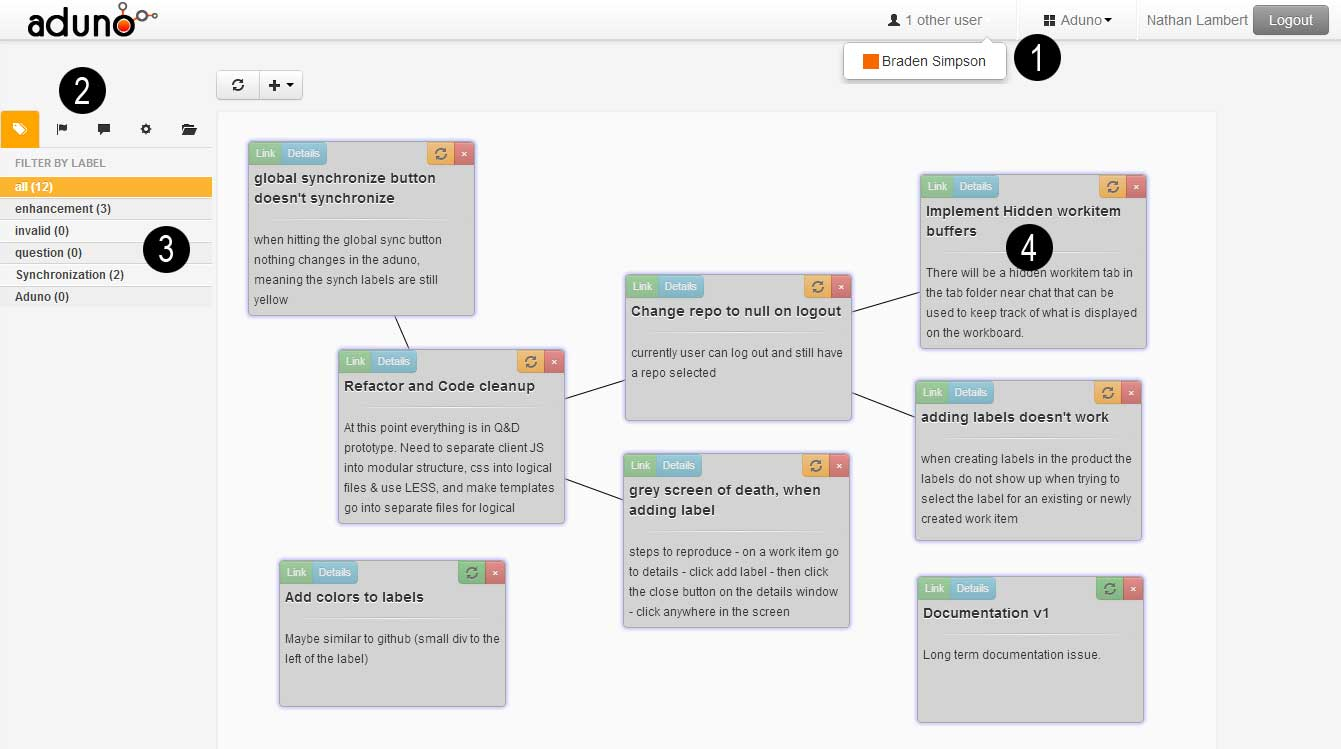
\includegraphics[width=\textwidth]{aduno-screenshot}
\caption{Aduno Screenshot}
\label{fig:adunoscreenshot}
\end{figure*}

\begin{table}[h]
\begin{center}
\begin{tabular}{@{\hspace{.2cm}}ccc@{\hspace{.2cm}}c@{\hspace{.2cm}}c@{\hspace{.2cm}}c@{\hspace{.2cm}}c@{\hspace{.2cm}}}
\hline
Similar Services&  Real-time&   Control of&  Tags&    Visual layout&      Chat&\\
 & & WorkItems& & & &\\
\hline
GitHub Issues   &	-&	        \cmark&	                \cmark& -&                  -\\ 
Google Code     &   -&          \cmark&                 -&      -&                  -\\
Jazz            &   -&          \cmark&                 \cmark& -&             -    \\
Aduno           &   \cmark&     \cmark&                 \cmark& \cmark&             \cmark\\
\hline
\end{tabular}
\end{center}
\caption{Comparing Collaborative Tools\label{tab:services}}
\label{tab:otherservices}
\end{table}

Other collaborative development environments (CDEs) have some of their features mapped in Table~\ref{tab:otherservices}.  They provide an almost exclusively asynchronous approach to developing articulative work, and this is one of the motivators for Aduno.  Aduno poses to interface with these other CDEs and create functionality to create semi-synchronous collaborative experience.  GitHub was chosen as the preferred backend because of it's robust and open API, in addition to it hosting almost three million open-source repositories.

\subsection{Purpose}
Aduno was constructed around the requirements described in Section~\ref{sec:pdesign}.  From this model, the requirements were gathered and formulated into implementation.  The main aspects of collaborative applications that were the basis of the architectural design decisions of Aduno are \emph{speed}, \emph{synchronicity}, and \emph{simplicity}.  With these components in mind, the development team built Aduno to be able to interface with the GitHub API, or other RESTful services, to provide a faster, more effective way to collaborate on articulative tasks. 

\subsection{Architecture}
With \emph{speed} being one of the most important aspects of the design, the architecture chosen for the server-side technology is crucial.  Node.js\footnote{A platform for building fast, scalable network applications, http://nodejs.org}, a platform of server-side JavaScript built on Google Chrome's V8 JavaScript runtime, was chosen as our platform.  Node has been quickly adopted as a powerful platform for web applications such as Cloud9\footnote{A collaborative web IDE built in Node.js}, LinkedIn, Windows Azure and more.  Tilkov \& Vinoski~\cite{TV10} have shown Node as a viable choice for non-blocking web applications.  Using Node allows Aduno to be deployed easily to the Amazon Elastic Cloud compute instances as a cloud service, which offers reliability and scalability.

\emph{Synchronicity} is a crucial component of Aduno and was a great influence over the frameworks chosen for the tool.  The Meteor Framework\footnote{An open-source web application framework focused on real-time updates} was chosen to support asynchronous data among users, since Meteor pushes changes out to clients dynamically, updating their screens without refreshing, and unobtrusively keeping users synchronized.  

\emph{Simplicity} is a key point in any application that needs to attract its new users, and Aduno had this principle as a top priority.  The web toolkit used to support this is Twitter Bootstrap, a very common open-source user interface toolkit, with approximately 100 developers.

\subsection{Feature Description}
Figure~\ref{fig:adunoscreenshot} shows a typical example of Aduno's interface, with a few emphasized features: {\bf (1)} The top navigation bar with a menu to select the repository to work on, and an indicator showing other online collaborators. {\bf (2)} Tabbed workflow panel that lets users switch between label list, milestone list, and chat area. {\bf (3)} Label filters that let users show only specific work items based on a specific label {\bf (4)} Work items that can be edited in real-time by several users. They can be linked to other work items, as shown in the screenshot. This allows for a visual representation of links, which is not offered by other services.

Although it is typical for project management systems in services such as GitHub to allow comments on each issue (herein referred to as the more generic term \textit{work item}), we have included a chat area in Aduno. The comments on work items in Github are used for asynchronous communication, and this was not sufficient for our tool. A chat system provides users with a secondary communication channel that allows them to engage in a semi-synchronous discussion about work items that would not typically be appropriate for asynchronous work item comments. Since comments in Github must also be attached to only one work item, having this chat area helps teams develop broader goals and facilitates common ground through more in-depth conversation.

As noted on Figure~\ref{fig:adunoscreenshot}, one of the paramount features of Aduno is the ability to organize work items on the workboard (the "canvas" on which the work items are displayed). In other services, work items are displayed in a list without any notion of priority. Although they allow for links between work items, users must follow a link to view the other work items. Having a visual representation of the links allows users to quickly glance at the related work items. Allowing users to move the work items around on the work board gives them several opportunities, including being able to arrange them in whatever context that seems appropriate at the time. Work items may be ordered chronologically, in order of importance, or in whatever order the team wishes. Work items may not only be linked, but they may also be grouped together to imply a connection. Links are part of the Aduno API, so they can be passed on to any associated services that support this feature, such as GitHub.

When an edit is performed on a work item in Aduno, the "Sync" indicator at the top right of the item turns from green to orange to signal that there is an unsynchronized change. To synchronize with GitHub, the user may click on the Sync All button at the top of the page, or they may click on a work item's Sync button to synchronize it individually. This gives the team more control over what work items get synced with the associated service.

The elements of workspace awareness outlined in Table~\ref{tab:Gutwin} should be completely fulfilled in an effective collaborative application, although some of them are not applicable to this tool. As previously mentioned, awareness of gaze, view, and reach would add much complexity to the tool without providing much benefit. However, the remaining elements play an important role in user awareness with Aduno.
  
{\bf Presence} – An indicator in the navigation bar at the top of the screen signals the presence of other users.  Also, whenever users are interacting with controls in the workspace, they have their presence made in the form of their unique color and username badge shown.

\begin{figure}[htb]
\centering
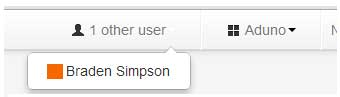
\includegraphics[scale=0.5]{aduno01}
\caption{Online user indicator}
\label{fig:otherusers}
\end{figure}

{\bf Identity} – Clicking on the indicator shows a dropdown listing of all the current online users. A color unique to that user is displayed next to their name.  This is a globally used identity that is persistent to all items related to the user. 

{\bf Authorship} – When a user is editing a work item, their name is displayed at the bottom of it to indicate that they are currently working on it.

\begin{figure}[htb]
\centering
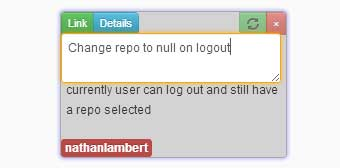
\includegraphics[scale=0.5]{aduno02}
\caption{Work Item Being Edited}
\label{fig:workitem}
\end{figure}

{\bf Action} – Editing actions result in real-time data propagation, immediately showing changes across all clients that are connected to the same repository.  

{\bf Intention} – The intention of most work item edits would likely be apparent as the edits are being done. Broader goals may be discussed in the chat window. A markdown language is used on the chat to provide contextual awareness to the users.  For example someone can reference a work item by using it's ID in the chat window.
 
{\bf Artifact} – As shown in Figure~\ref{fig:workitem}, usernames are displayed at the bottom of it to indicate that they are currently working on an item.

{\bf Location} – The location of the user’s work is shown by the username attached to a work item when they are doing edits. If the user moves a work item around, their location becomes apparent.

{\bf Ownership} - Storing a history of modifications to work items is a way to add awareness for users that are not synchronously working, and allows for reflection on the creation process.

\section{Evaluation}

To evaluate Aduno's usability and fit for the intended use, we carried out an expert judgement study involving eight users, forming four pairs. The experts had experience in distributed software development ranging from one to ten years and have participated in multiple collaborative projects.

\subsection{Setup}
The experts were invited to participate in the evaluation session and, after indicating their availability, were randomly assigned to pairs. In each evaluation session, the experts were first given a short demonstration of the tool's features and the shared workspace layout. Following that, participants were given a short description and high-level requirements for a fictional website they would have to build. They were asked to use the tool to collaboratively define and link work items. The experts were not allowed to communicate outside the tool, as a way to account for them being distributed. For the final part of the evaluation session, experts were given a short questionnaire to fill out, evaluating the tool's fulfillment of its purpose as well as its potential impact on a project.

\subsection{Results}
\label{sec:results}
\begin{table*}[t]
\begin{center}
\begin{tabular}{@{\hspace{.2cm}}llll@{\hspace{.2cm}}c@{\hspace{.2cm}}c@{\hspace{.2cm}}c@{\hspace{.2cm}}}
\hline
Collaborative Behaviours&  Mean&   Median&  St. Dev.&\\
\hline
Visualizing work items& 4.125& 4& 0.83\\
Brainstorming& 3.375& 4& 1.19\\
Translating ideas to actionable items& 4& 4& 1.07\\
Ease to use& 4& 4& 0.75\\
Ease to learn& 4.75& 5& 0.46\\
Ease to integrate with current workflow& 3.875& 4& 0.83\\
\hline
Importance of Awareness& 4.375& 4.5& 0.77\\
Satisfaction with Awareness& 3.5& 3& 0.92\\
\hline
Importance of Connection& 3.875& 4& 1.12\\
Satisfaction with Connection& 3.25& 3& 1.03\\
\hline
Importance of Transmission& 3.625& 4& 1.5\\
Satisfaction with Transmission& 3.625& 3.5& 0.74\\
\hline
Importance of Notification& 3.25& 3& 1.03\\
Satisfaction with Notification& 2.5& 2.5& 1.19\\
\hline
Importance of Ownership& 3.375& 3.5& 1.4\\
Satisfaction with Ownership& 3& 3.5& 1.19\\
\hline
Importance of Common Ground& 4.25& 4& 0.7\\
Satisfaction with Common Ground& 3.5& 3.5& 0.92\\
\hline
Importance of Responsiveness& 4.5& 5& 0.75\\
Satisfaction with Responsiveness& 2.75& 2& 1.39\\
\hline
Importance of Shared Information Space& 4.375& 5& 0.91\\
Satisfaction with Shared Information Space& 3.875& 4& 1.12\\
\hline
\end{tabular}
\end{center}
\caption{Collaborative behaviours and coordination}
\label{tab:surveyresults}
\end{table*}

Overall, Aduno impressed the experts and received positive feedback. The results of the expert study are shown in Table~~\ref{tab:surveyresults}. 
%TODO Table with stats
Aduno was considered a useful tool, especially for visualizing work items, while the experts also appreciated Aduno's ease to learn, use, and integrate into their current workflow.

The experts were asked to rate the importance of Clark's \cite{Clark96} collaborative behaviors (adapted for software development), as well as their satisfaction with Aduno's support for each of them. Experts ranked \textit{maintaining awareness} and \textit{sharing an information space} as the most important elements for collaborative software development tasks. Given the frameworks we reviewed in Section~\ref{sec:intro}, this is not a surprising demand for a {\sc cscw} tool. At the same time Aduno also scored high in terms of the experts' satisfactions with supporting these elements. Establishing common ground was also one of the demands of the experts that Aduno successfully fulfills. 

In addition to the closed-ended questions, the experts were asked to evaluate Aduno's potential impact on a team's productivity in a real project. Six out of eight respondents indicated that they expect a positive impact, especially in terms of offering transparency during the design phase. The experts also commented on the ability to have commonly agreed on tasks, and how this positively affects the structure and organization of the project. The remaining two experts recognized Aduno's potential but would like it to cater to larger groups and be more explicit with milestones to have a strong positive effect.

Regarding challenges, the experts were only concerned with the scalability of Aduno and whether it will be able to support large groups and a large number of work items. Participants were also asked to provide suggestions and improvements for future development on Aduno, which will be discussed in Section~\ref{sec:future}.

\section{Future Work}
\label{sec:future}
Future work for Aduno will be carried out on two levels: extending the tool's features based on the experts' feedback, and doing quantitative evaluation. 
\subsection{Development}
During this study Aduno has been evaluated using an experts evaluation, which has provided a large amount of feedback for the development team and has highlighted many new features.  Apart from small user interface improvement suggestions, the main points of interest were as follows:

\begin{itemize}
    \item{More robust support for large number of work items}
    \item{Stronger chat Features} 
    \item{More robust API mapping to GitHub}
\end{itemize}

Although this input from the expert evaluators is extremely useful, these types of feature requests were anticipated due to the prototypical nature of the tool.  The future work on Aduno will include a significant amount of development in these areas, as well as potentially interfacing the backend with another service such as IBM Jazz\footnote{Project lifecycle management tools by IBM -- https://jazz.net/story/about}, or Atlassian Jira\footnote{Production grade project tracking system -- http://atlassian.com/software/jira/overview}. Due to the modular design of the Aduno API, the developers can easily plug in new services.  

Larger teams is another focus of the future development.  As shown in Section~\ref{sec:results}, the results of the evaluation were positive, but the experts wanted a lot more support for larger projects -- or more work items to be seen at once.  This is a crucial feature for Aduno that has to, and will be addressed.  The implementation could include a zoomable workboard, which could act as a map that can be scrolled and interacted with.   

\subsection{Evaluation}
We plan to do a more extensive evaluation of Aduno in terms of user engagement, and also perform a quantitative analysis to investigate how its use affects team productivity. One idea to attract more users for our evaluation is to import data from their projects on GitHub into Aduno and then contact them with a demo of the tool with their own data. This approach will motivate the team by giving them a real data snapshot of their issue tracker already running in Aduno and can instantly show them the value of the tool.  With regard to the quantitative study, we plan to assess the impact of Aduno's use on a team's speed and the need for clarification. Since Aduno helps the team collaboratively define and link work items, especially during the initial stages of the project, we expect less time spent for clarifications in later stages of development and an increase in development speed associated with that. We aim towards consistently supporting the development team through their articulation work and, as a result, minimize the timespan for clarification activities and increase their productivity.

\subsection{Conclusion}
In this paper we introduced Aduno, a real-time collaborative tool for defining and managing work items in distributed software development teams. The aim behind the tool is to support workspace awareness and common ground during the initial stages of development when it is critical for a team to collaboratively make design decisions and translate them into actionable items. The tool's features cover the major requirements for collaborative applications as they are known from the {\sc cscw} literature, and have been evaluated by experts. Our future plans for the tool include expanding the feature list as well as doing a quantitative evaluation to measure its impact on team productivity.

\bibliographystyle{IEEEtran} 
\bibliography{aduno}

\end{document}
